\section{Introducción}

La red que se ha elegido para realizar esta práctica es la de \textit{Political
blogs}~\cite{data} de la
\href{http://www-personal.umich.edu/~mejn/netdata/}{página web de
Mark Newman}. Como su propio nombre indica, se trata de una red de blogs sobre
política de los Estados Unidos de América, donde los nodos son los blogs y las
aristas, los enlaces de una web a otra, tratándose entonces de un grafo
dirigido.

En la figura~\ref{fig:network-parties} se puede ver la representación gráfica de
la red. Como se puede apreciar, la red se ve muy pequeña, esto se debe a que hay
muchos nodos que no tienen relación con ningún otro, de manera que están
aislados. En la figura, estos nodos forman un círculo casi imperceptible
alrededor de la componente principal.

\begin{figure}[h!]
    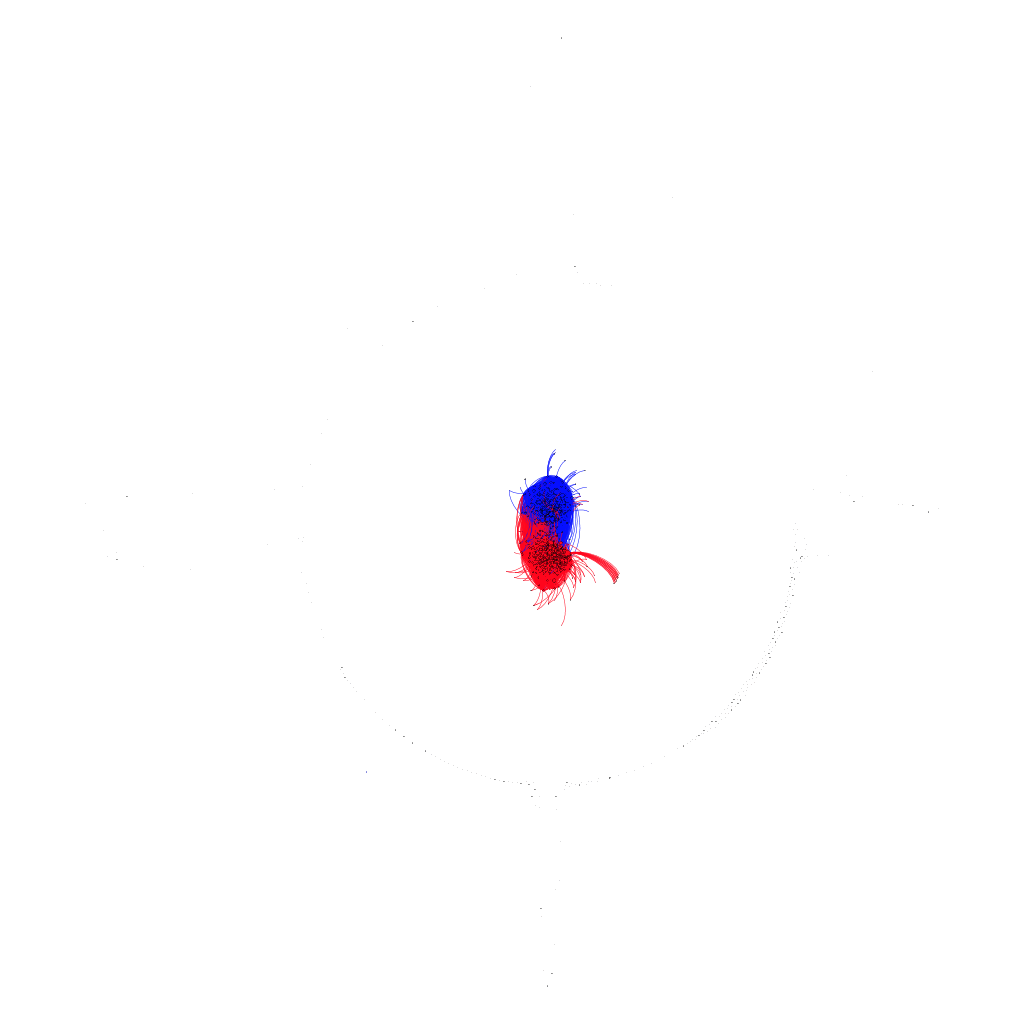
\includegraphics[height=\textwidth]{images/network/parties.png}
    \caption{Representación gráfica de la red}
    \label{fig:network-parties}
\end{figure}

\newpage

Si filtramos la red para quedarnos solo con esta componente gigante, obtenemos
el grafo de la figura~\ref{fig:network-giant-component}, que es mucho más
apreciable. Se han utilizado los colores clásicos para representar las
ideologías políticas en los EEUU: el azul para la izquierda o los liberales y el
rojo para la derecha o los conservadores. El tamaño de un nodo refleja el grado
total del mismo, de forma que los nodos más grandes representan blogs que
realizan/reciben más enlaces. Como era de esperar, los blogs de cada ideología
están fuertemente agrupados entre ellos, habiendo también bastantes referencias
de algunos blogs de cada ideología hacia la otra.

\begin{figure}
    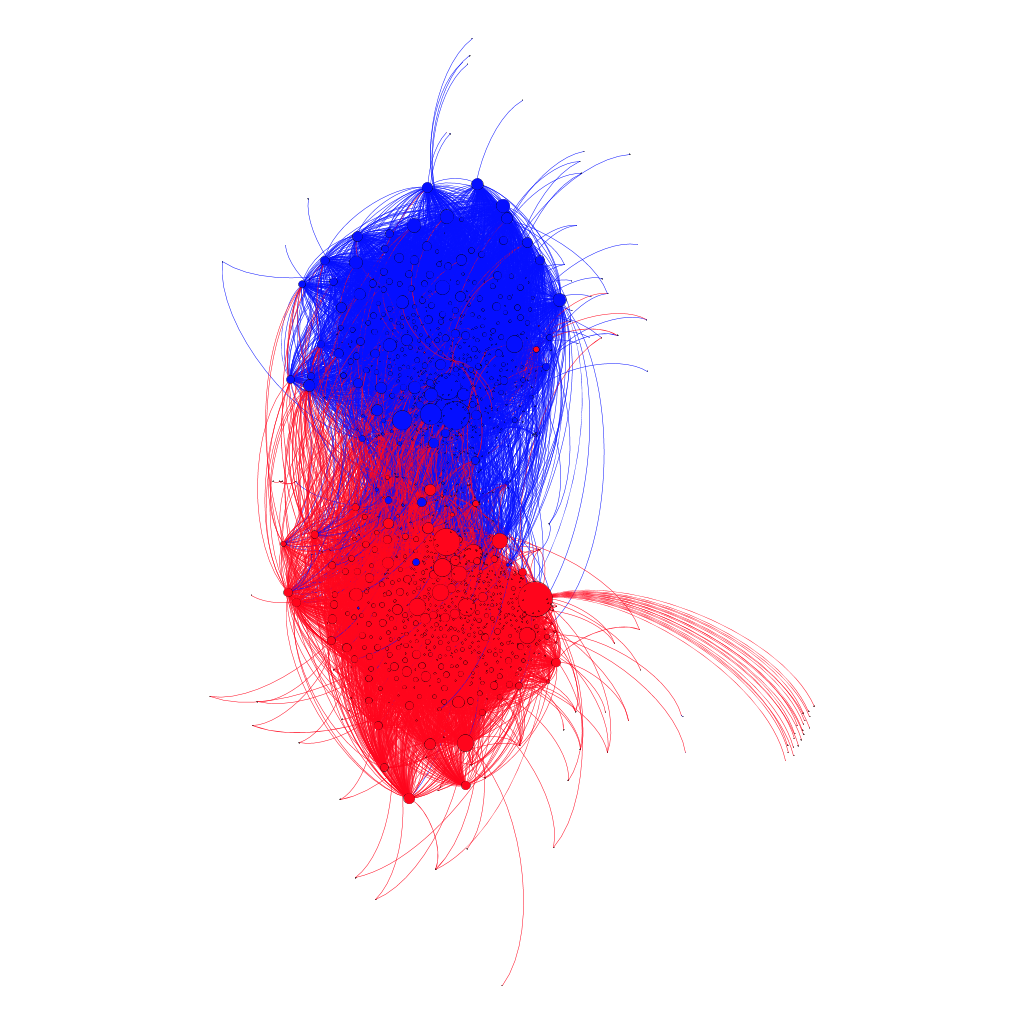
\includegraphics[width=\textwidth]{images/network/giant-component.png}
    \caption{Representación gráfica de la componente gigante}
    \label{fig:network-giant-component}
\end{figure}
